\documentclass[UTF8]{ctexart}
\usepackage{graphicx}
\usepackage{ctex}
\usepackage{tikz}
\usepackage{amsmath}
\title{热力学与统计物理-第三次作业}
\author{吴远清-2018300001031}

\begin{document}
	\maketitle
	1.17\\
	We can treat this as biominal distribution: Each molecules only have two states: In the volume or not. The probability of the molecules in the volume is:
	$$p = \frac{V}{V_0} \eqno(1.1)$$
	Then, use  Gaussian approximation:
	$$P(N) = (2\pi N_0 p q)^{-\frac{1}{2}}exp[-\frac{(N - N_0 p)^2}{2N_0 p q}]\eqno(1.2)$$
	So, we can get the result:
	$$P(N,N+dN) = \int_{N}^{N+dN}(2\pi N_0 p q)^{-\frac{1}{2}}exp[-\frac{(N - N_0 p)^2}{2N_0 p q}]dN$$
	$$= (2\pi N_0 p q)^{-\frac{1}{2}}exp[-\frac{(N - N_0 p)^2}{2N_0 p q}]dN$$
	$$= (2 \pi N_0 \frac{V (V_0 - V)}{V_0^2})^{-\frac{1}{2}}exp[-\frac{(V_0 N - N_0 V)^2}{2N_0 V (V_0 - V)}]dN \eqno(1.3)$$
	
	1.18\\
	Answer:\\
	This question equal to the off-latice 3D random walk.\\
	For each step, we have the constant length l, and a random direction that can be described by $\theta,\phi,\, \theta$ is the angle between the projection of direction vector on XY plane and the X positive semi-axis, and $\phi$ is the angle between the direction vector and XY plane. For N steps:
	$$\{\theta_1,\theta_2,...,\theta_N,\phi_1,\phi_2,...,\phi_N\}\eqno(2.1)$$
	Then, we have:
	\begin{equation*}
	\left\{
	\begin{aligned}
	&\overline{r_x^2} = \overline{l^2 \times \sum_{i=1}^{N}(cos^2\phi_i cos^2\theta_i)} = l^2 \times N \times \overline{cos^2\phi cos^2\theta}\\
	&\overline{r_x^2} = \overline{l^2 \times \sum_{i=1}^{N}(cos^2\phi_i sin^2\theta_i)} = l^2 \times N \times \overline{cos^2\phi sin^2\theta}\\
	&\overline{r_z^2} = \overline{l^2 \times \sum_{i=1}^{N}(sin^2\phi_i)} = l^2 \times N \times \overline{sin^2\phi}
	\end{aligned}
	\right.\eqno(2.2)
	\end{equation*}
	Using the periodicity of triangle function:
	\begin{equation*}
	\left\{
	\begin{aligned}
	&\overline{cos^2\theta} \,=\, \int_{0}^{2\pi}cos^2\theta d\theta \,=\, \frac{1}{2} + 	\frac{1}{2}\int_{0}^{2\pi}cos(2\theta)d\theta \,=\, \frac{1}{2}\\
	&\overline{sin^2\theta} \,=\, \int_{0}^{2\pi}sin^2\theta d\theta \,=\, \frac{1}{2} - \frac{1}{2}\int_{0}^{2\pi}cos(2\theta)d\theta \,=\, \frac{1}{2}
	\end{aligned}
	\right.\eqno(2.3)
	\end{equation*}
	Same for $\phi$, $\phi$ and $\theta$ are independent variable, so:
	\begin{equation*}
	\left\{
	\begin{aligned}
	&\overline{cos^2\phi cos^2\theta} = \overline{cos^2\phi} \times \overline{cos^2\theta}\\
	&\overline{cos^2\phi sin^2\theta} = \overline{cos^2\phi} \times \overline{sin^2\theta}
	\end{aligned}
	\right.\eqno(2.4)
	\end{equation*}
	Substitute (2.4), (2.3) into (2.2):
	\begin{equation*}
	\left\{
	\begin{aligned}
	&\overline{r_x^2} = \frac{N}{4} l^2\\
	&\overline{r_y^2} = \frac{N}{4} l^2\\
	&\overline{r_z^2} = \frac{N}{2} l^2
	\end{aligned}
	\right.\eqno(2.5)
	\end{equation*}
	Finally, we get:
	$$\overline{r^2}\,=\,\overline{r_x^2}+\overline{r_y^2} + \overline{r_z^2}= N \times l^2\eqno(2.6)$$
	2.1 \\
	Answer:\\
	For this particle, all of its energy is kinetic energy, so we have:
	$$P = \sqrt{2mE}\eqno(3.1)$$
	And the classical phase space is:
	\begin{figure}[h]
		\centering
		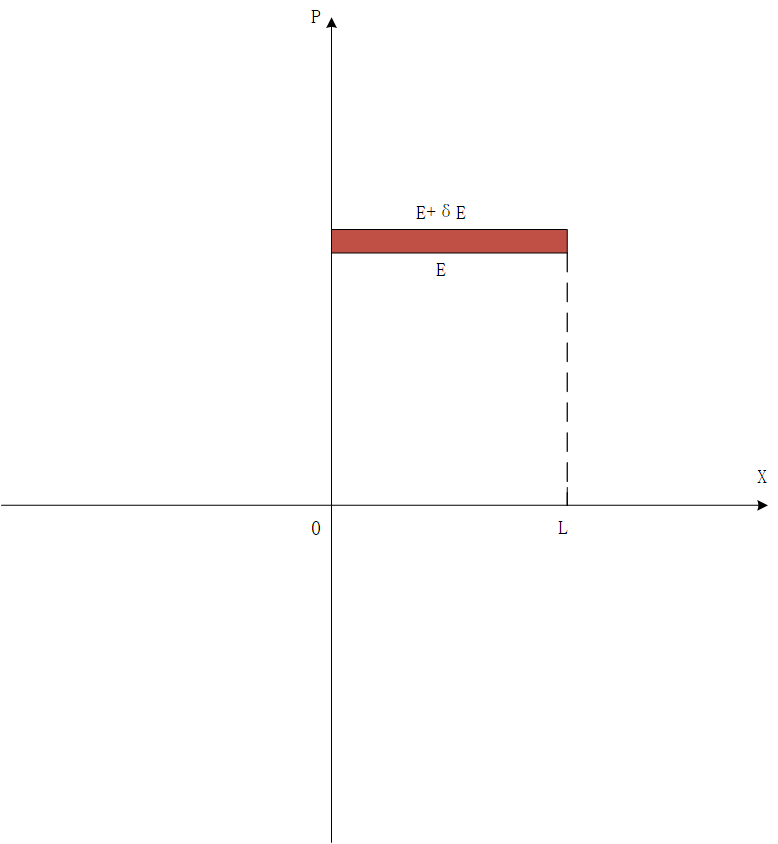
\includegraphics[scale=0.5]{3-1.png}
		\caption{Classical phase space}
	\end{figure}
	
	2.4 \\
	Answer:\\
	(a). The energy of the system is:
	$$E = -(n_1 - n_2)\mu H = -(2n_1 - N)\mu H\eqno(4.1)$$
	So:
	$$n_1 = \frac{N}{2} - \frac{E}{2 \mu H} \eqno(4.2)$$
	Since $\delta E$ is very small compared to E:
	$$\Omega(E) = \int_{E}^{E + \delta E}\Omega(E')dE' \approx \Omega(E)\delta E = \Omega(n_1)\delta n_1 \eqno(4.3)$$
	From (4.2):
	$$\delta n_1 = \frac{\delta E}{2\mu H}\eqno(4.4)$$
	Then:
	$$\Omega(E) = \frac{N!}{n_1!(N-n_1)!}\frac{\delta E}{2\mu H} = \frac{N!}{(\frac{N}{2} - \frac{E}{2 \mu H})!(\frac{N}{2} + \frac{E}{2 \mu H})!} \frac{\delta E}{2\mu H} \eqno(4.5)$$
	(b) From (4.5):
	$$ln \, \Omega(E) = ln \, N! - ln \, (\frac{N}{2} - \frac{E}{2 \mu H})! - ln \, (\frac{N}{2} + \frac{E}{2 \mu H})! + ln \, \frac{\delta E}{2\mu H} \eqno(4.6)$$
	With Stirling's formula:
	$$ln \, n! \approx n \, ln \, n - n \eqno(4.7)$$
	(4.6) aprroximate to:
	$$ln \, \Omega(E) =  N \, ln \, N - (\frac{N}{2} - \frac{E}{2 \mu H}) \, ln \, (\frac{N}{2} - \frac{E}{2 \mu H})$$
	$$ - (\frac{N}{2} + \frac{E}{2 \mu H}) \, ln \, (\frac{N}{2} + \frac{E}{2 \mu H}) + ln \, \frac{\delta E}{2\mu H}\eqno(4.8)$$
	(c) For this system, the spin is parallel or antiparallel have an equal probability. So:
	$$P(n_1) = (\frac{1}{2} \pi N)^{-\frac{1}{2}}exp[-\frac{(n_1-\frac{N}{2})^2}{\frac{N}{2}}] \eqno(4.9)$$
	Consider (4.2):
	$$P(E) = (\frac{1}{2} \pi N)^{-\frac{1}{2}}exp(-\frac{E^2}{2 N \mu^2 H^2})\eqno(4.10)$$
	So, the $\Omega(E)$ is:
	$$\Omega(E) = P(E) \times 2^N = 2^N (\frac{1}{2} \pi N)^{-\frac{1}{2}}exp(-\frac{E^2}{2 N \mu^2 H^2})\eqno(4.11)$$
	
	2.7  \\
	Answer:\\
	(a). The energy's change is:
	$$\Delta E = E(L_x + dL_x) - E(L_x) \eqno(5.1)$$
	The change of system energy is equal to the negative value of system work to the outside:
	$$W = - \Delta E \eqno(5.2)$$
	The system's work to outside given by:
	$$W = \int_{L_x}^{L_x + dL_x}F_x(x')dx' \approx F_xdL_x \eqno(5.3)$$
	Since $dL_x$ is a small amount, The approximation in the above formula can be satisfied. Then, from (5.1) to (5.3), we can get:
	$$F = -\frac{E(L_x + dL_x) - E(L_x)}{dL_x} = - \frac{\partial E}{\partial L_x} \eqno(5.4)$$
	Q.E.D
	(b). The energy of this particle is given by:
	$$E = \frac{\hbar^2}{2m}\pi^2 (\frac{n_x^2}{L_x^2} + \frac{n_y^2}{L_y^2} + \frac{n_z^2}{L_z^2})\eqno(5.5)$$
	Then we can calculate the force that particle exert on the wall:
	\begin{equation*}
		\left\{
		\begin{aligned}
			&F_x = 2\frac{\hbar^2}{2m^2}\pi ^2 \frac{n_x^2}{L_x^3}\\
			&F_y = 2\frac{\hbar^2}{2m^2}\pi ^2 \frac{n_y^2}{L_y^3}\\
			&F_z = 2\frac{\hbar^2}{2m^2}\pi ^2 \frac{n_z^2}{L_z^3}
		\end{aligned}
		\right.\eqno(5.6)
	\end{equation*}
	Then we can calculate the pressure on three direction:
	\begin{equation*}
	\left\{
	\begin{aligned}
	&P_x = 2\frac{\hbar^2}{2m^2}\pi ^2 \frac{n_x^2}{L_x^2V}\\
	&P_y = 2\frac{\hbar^2}{2m^2}\pi ^2 \frac{n_y^2}{L_y^2V}\\
	&P_z = 2\frac{\hbar^2}{2m^2}\pi ^2 \frac{n_z^2}{L_z^2V}
	\end{aligned}
	\right.\eqno(5.6)
	\end{equation*}
	The total pressure is:
	$$P = \frac{P_x + P_y + P_z}{3} = \frac{2}{3V}\frac{\hbar^2}{2m^2}\pi^2(\frac{n_x^2}{L_x^2} + \frac{n_y^2}{L_y^2} + \frac{n_y^2}{L_y^2}) \eqno(5.7)$$
	The average is:
	$$\bar{P} = \frac{2}{3}\frac{\bar{E}}{V} \eqno(5.8)$$
	
	2.10 \\
	Answer:\\
	We can treat $\bar{P}$ as a function of V:
	$$\bar{P} = KV^{-\gamma} \eqno(6.1)$$
	Since the wrok is done through a quasistatic process, we can divided the change of volume into three dimension's length change, here we only consider X direction, the other two directions will be same and easy to prove:
	$$F_x = \bar{P_x} S_x \eqno(6.2)$$
	$$W = \int_{X_s}^{X_f}F_xdx = \int_{X_s}^{X_f}K(S_x X)^{-\gamma}S_xdx = KS_x^{-\gamma + 1}\int_{X_s}^{X_f}X^{-\gamma}dx \eqno(6.3)$$
	Then:
	$$W = -K(\gamma - 1)(V_f^{-\gamma + 1} - V_s^{-\gamma + 1}) \eqno(6.4)$$
	Replace K with $\bar{P_s}V_s^\gamma$:
	$$W = -\bar{P_s}V_s^\gamma(\gamma - 1)(V_f^{-\gamma + 1} - V_s^{-\gamma + 1}) \eqno(6.5)$$
	
	2.11.\\
	Answer:\\
	First, we'll calculate the difference of internal energy between state A and B.
	$$\Delta E = -W = \int_{V_A}^{V_B}\bar{P}dV = \int_{V_A}^{V_B} \alpha V^(-5/3)dV = -3600 J \eqno(7.1)$$
	(a).\\
	$$W = \int_{V_A}^{V_{B'}}\bar{P}dV = 22400 J \eqno(7.2)$$
	With the first law:
	$$\Delta E = Q - W = -3600 J \eqno(7.3)$$
	$$Q = 18800 J \eqno(7.4)$$
	(b)\\
	$$W = \int_{V_A}^{V_B}\bar{P}dV = 11500 J\eqno(7.5)$$
	From (7.3):
	$$Q = 7950 J \eqno(7.6)$$
	(c)\\
	$$W = \int_{V_A'}^{V_B}\bar{P}dV = 700 J \eqno(7.7)$$
	From (7.3):
	$$Q = -2900 J \eqno(7.8)$$
	
	
\end{document}